\documentclass[arial,11pt]{article}
%\documentclass[11pt]{nih}
\usepackage[dvips]{graphicx}
\usepackage[colorlinks=true,linkcolor=black]{hyperref}
\usepackage{amssymb}
%\usepackage{graphicx}
%\usepackage{longtable}
\usepackage{epsfig}
%\usepackage{overcite}
\usepackage[usenames]{color}

\renewcommand{\rmdefault}{phv} % Arial
\renewcommand{\sfdefault}{phv} % Arial
\renewcommand{\thesection}{\Alph{section}}
\pagestyle{empty}

%\usepackage{times}
\usepackage{geometry}
%\geometry{tmargin=1in,bmargin=1.0in,lmargin=1in,rmargin=1in}
\geometry{tmargin=0.95in,bmargin=0.95in,lmargin=0.95in,rmargin=0.95in}
%\linespread{0.95} \interfootnotelinepenalty=10000

%%%%% editing helpers
\newcommand{\NeedRevision}[1]{\textcolor{red}{#1}}

\begin{document}

\begin{center}
\Large
{\bf Driving Biomedical Project 4:\\A systems approach towards the therapeutic modulation of the acetylome}
\normalsize
\end{center}

\begin{itemize}
%\item {\bf Funding status of the project:}  funded
\item {\bf Collaborating investigator:}  Anne-Claude Gingras
\item {\bf Institution:} Samuel Lunenfeld Research Institute, Toronto, Canada
\item {\bf Funded project:} 	A Systems Approach Towards the Therapeutic Modulation of the Acetylome
\item {\bf Grant number:} 	275594   	
\item {\bf Project period:}   9/1/2012 to 8/31/2016
\item {\bf Agency:}  CIHR/IRSC (Canada)
\item {\bf TRD interactions:}  TRD3 (Spectral networks), TRD4 (Universal MS tools), TRD7 (Multiplexed spectra) and TRD8 (ProteoSAFe, MassIVE).
\end{itemize}
%  \begin{tabular}{rl}
%  Collaborating PI(s): & Anne-Claude Gingras, Ph.D. \\
%  Institution: & Samuel Lunenfeld Research Institute, Toronto, Canada \\
%  Funding: \\
%    CIHR/IRSC & 275594, Sep 2012 to Aug 2016, PI Gingras
%  \end{tabular}
%\ \\\ \\
%{\bf TRD interactions: } TRD3 (Spectral networks), TRD4 (Universal MS tools), TRD7 (Multiplexed spectra) and TRD8 (ProteoSAFe/MassIVE).

%*******************************************
\section{Significance}
%*******************************************

%(1) Significance:
%\begin{itemize}
% \item address the importance as an impetus for TR\&D of the biomedical research problem that will form the basis of the DBP;
% \item challenges inherent in this research problem that will drive TR\&D;
% \item appropriateness of the DBP as a test-bed for technology being developed in the BTRC.
%\end{itemize}

The cellular machinery responsible for the acetylation of lysines is critically implicated in cancer biology. In particular the only protein domain that recognizes acetylated lysines, the bromodomain, is present in multiple proteins implicated in chromatin biology and regulation of gene expression, and many of these proteins are deregulated in human tumors. The recognition of acetylated peptides by the bromodomain makes them an attractive druggable target~\cite{filippakopoulos12}.
%Through the work of one of the co-PIs associated with this DBP~\cite{muller11},
The first anti-cancer bromodomain inhibitor
%(JQ1; specific for the BET family of bromodomains)
has been developed and shows promise against a number of tumor types. However, this work also highlighted the need for more information regarding the cellular context in which bromodomain containing proteins and acetylation enzymes act, and what are the cellular targets for bromodomain recognition of acetylated peptides. This DBP aims to systematically define the specificity and function of human bromodomains through identification of their binding partners and acetylated targets.

{\bf The acetylation machinery (acetylome).} Lysine acetylation (KAc) is the process by which an acetyl group is transferred (from Acetyl Coenzyme A) to the epsilon amine of a lysine residue, a modification that is catalyzed by a family of lysine acetyltransferases (KATs). Similar to protein phosphorylation in which kinases and phosphatases~\cite{breitkreutz10} oppose each other for the addition ("writing") and removal ("erasing") of the phosphate group, KAc added by KATs can be removed by lysine deacetylases (KDACs). KAc marks are recognized by a single dedicated protein domain, the bromodomain, which acts as a "reader" of the acetylation mark and provides context-specific recognition.
% (44 genes in human; some proteins contain more than one bromodomain).
%Lysine acetylation first came to the forefront as a histone modification. Histone tails are modified by a number of post-translational modifications (PTMs) that present different cues to the cellular machinery (the so-called histone code). In general, acetylation of histone tails acts to open the chromatin structure, activating transcription, although certain acetylation marks are associated instead with chromatin compaction and with other processes as well, such as metabolism and DNA repair. However,
While first studied intensively in the context of the histone code, lysine acetylation is now recognized as a widespread post-translational modification (PTM) occurring on a large proportion of the proteome. So far, 18330 sites on 6870 proteins have been reported in total in human cells in a PTM repository (http://www.phosphosite.org), which is likely still an underestimation (new sites are regularly detected by mass spectrometry). The prevalence of KAc on thousands of cellular proteins underlies the vital importance of this modification and also highlights the lack of information regarding which KATs and KDACs are responsible for these acetylation events, and, just as importantly, which sites on which proteins are "read" by the different bromodomains.

{\bf Targeting the acetylome in disease.} Tight control of the acetylome is critical to cellular homeostasis, and many of the acetylome components have been associated with disease, particularly cancer~\cite{muller11}. The overexpression of multiple KDACs in cancers prompted the development and testing of KDAC (HDAC) inhibitors as anticancer therapeutics, and two of them (Voronistat and  Romidepsin) have been approved for the treatment of persistent or recurrent cutaneous T-cell lymphoma (CTCL). However, while these inhibitors show clear clinical promise, their cellular mode of action is still not clear. These compounds are also bound to be somewhat non-specific: besides the fact that most of the currently used inhibitors can target more than one KDAC, the number of direct acetylation targets for each of the KDACs (let alone their identity) is still largely unknown. Furthermore, most KDAC inhibitors have been shown in clinical trials to be ineffective as monotherapies, reinforcing the need for improved therapeutic agents targeting the acetylome. Given the more specific nature of the acetylation recognition, bromodomains are attractive drug targets. Bromodomain alterations in disease include expression changes, but also deletions, point mutations and translocations~\cite{muller11}. For example, translocations of the BET (Bromodomain and Extra Terminal domain) family members BRD4 and BRD3 to the NUT protein cause an aggressive midline carcinoma. Disrupting the KAc binding with the small molecule inhibitor JQ1 reverses the tumor phenotype of midline carcinoma cells, offering an excellent proof-of-concept for targeting protein-protein interactions for epigenetic "readers". Importantly, the anti-proliferative effects of JQ1 and other recently developed BET-family inhibitors extents beyond this rare malignancy, as BRD4 is critical for the growth of c-Myc driven cancers. As several other bromodomain-containing proteins are implicated in disease, there is a large ongoing effort for the development of additional specific inhibitors of the KAc-bromodomain interaction.
%, including in the unique industry/academic partnership led by the SGC (early access to newly developed compounds is provided through our collaborations; http://www.thesgc.org/scientists/epigenetics).

{\bf Recognition of acetylated lysines by bromodomains.} Despite variation in primary amino acid sequence, all bromodomains (a domain of 120 aa) share a common fold, and bind KAc in a similar manner.
%The bromodomain consists of a left-handed bundle of four alpha helices that are linked by more variable loop insert regions. KAc is recognized in a central deep and largely hydrophobic cavity, as determined by co-crystal structures of bromodomains complexed with KAc-containing peptides. Anchoring of the acetylated lysine (or lysines, see below) is provided by hydrogen bonding to a conserved asparagine residue.
How bromodomains specifically recognize distinct acetylated peptides is beginning to be understood, in large part due to the Gingras laboratory efforts to systematically determine the structures of multiple bromodomains. For example, while the structural fold of all bromodomains is similar, the electrostatic potential of the surfaces surrounding the KAc binding site is diverse, suggesting that they recognize different sequences.
% (e.g. positively charged histones may not be favored by bromodomains that have a positive charge, such as that of the first %bromodomain of PBRM1).
 Note that differences in surface charge have been observed even within the same protein, including the first and second domains of BRD4, suggesting that different bromodomains within a protein may target different sites.
%, an hypothesis that this project directly addresses for BRD4.
Additional selectivity elements are provided by the diverse loop regions that distinguish the different bromodomains.

\begin{figure}[ht!]
\centering
%  \vspace{-20mm}
    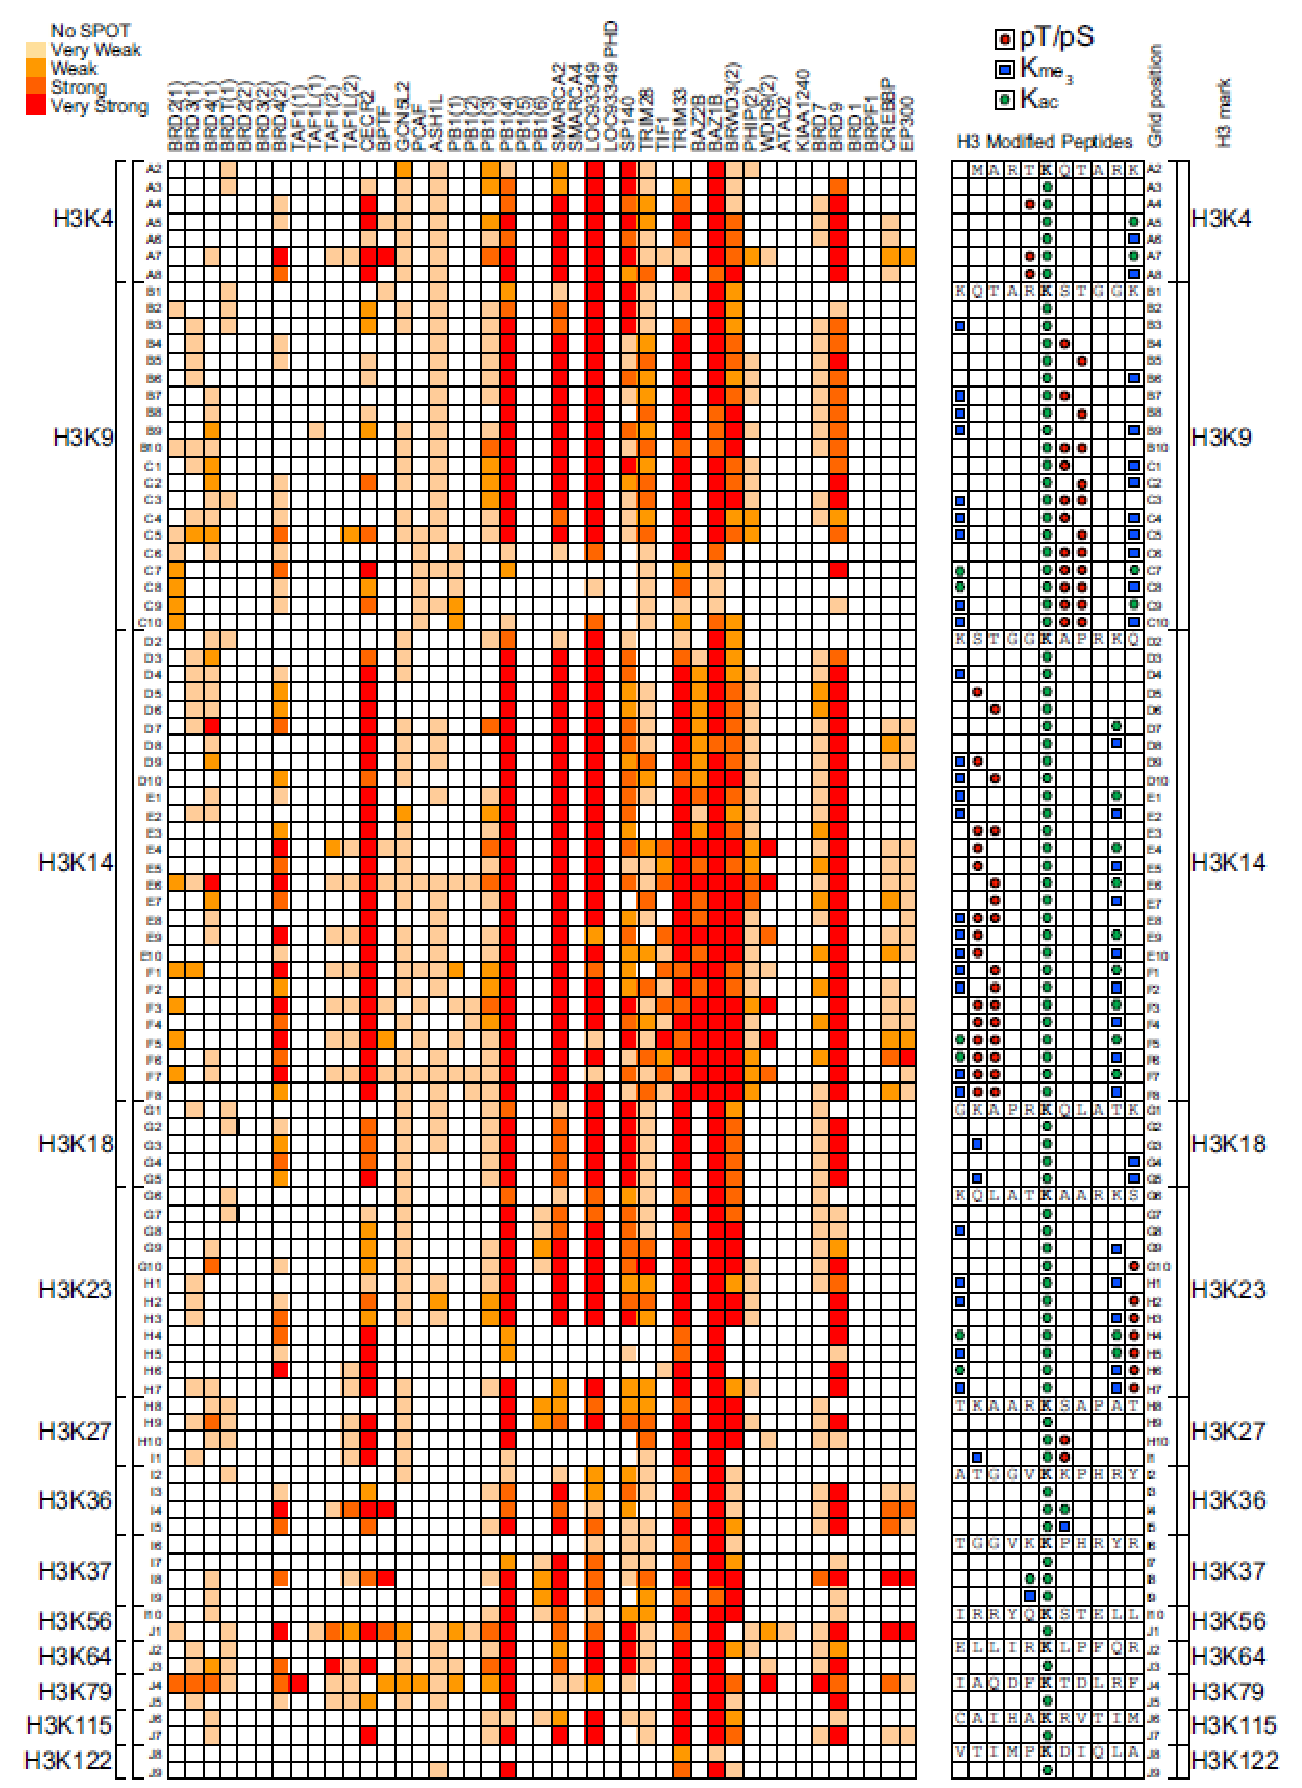
\includegraphics[width=.8\textwidth]{figures/BRDH3.pdf}
%    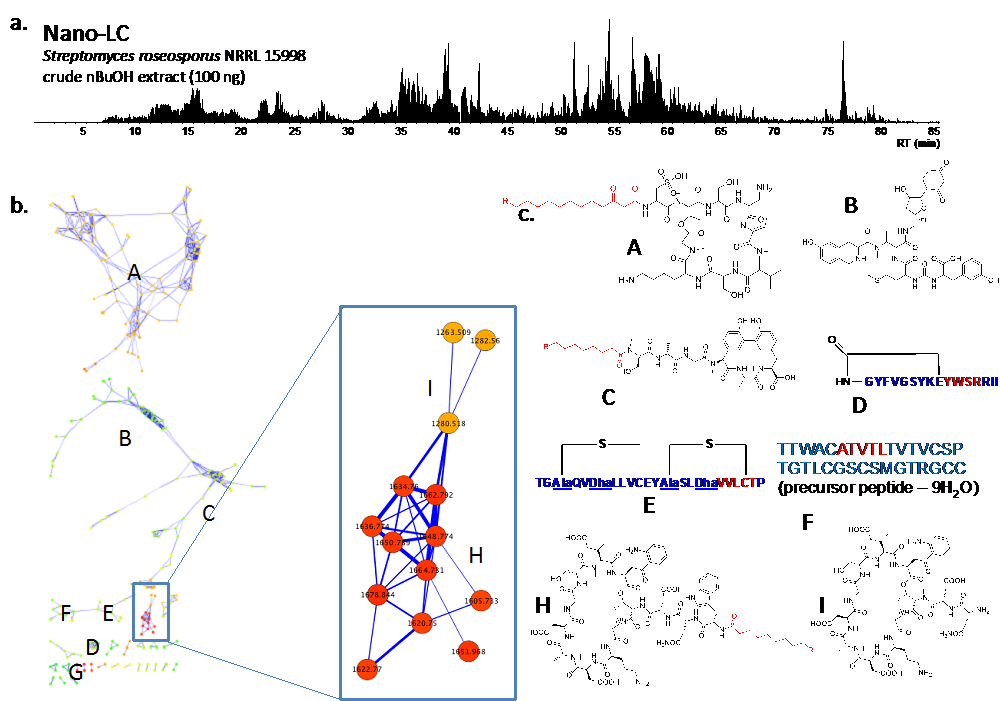
\includegraphics{figures/figApproach.png}
  \caption{\footnotesize {\bf Influence of Neighboring PTMs on BRD Interaction with Histone H3~\cite{filippakopoulos12}.} Shown are interactions shaded by spot intensity as indicated in the legend at the upper-left corner of the figure. The influence of lysine trimethylation (Kme3), acetylation, and phosphorylation (pT, pS) has been studied on binding to a central acetylated lysine epitope. The combination of the different modifications is indicated in the right panel. Nonmodified peptides have been included as controls to identify interactions independent of lysine acetylation. }
  \label{fig.dbp.gingras.ptms}
\end{figure}

{\bf How is the acetylome organized?} There is a pressing need to characterize systematically and in an unbiased manner the function of each of the components of the acetylation machinery and the relationships between the writer-reader-eraser modules. %As mentioned above, structurally, bromodomains offer attractive targets for therapies and are the topic of an intense drug discovery program, yet very little is known regarding the cellular context in which many of the bromodomain containing proteins reside or their specificity for their targets in vivo.
The Gingras laboratory used synthetic libraries of histone-derived peptides to provide information regarding the specificity of isolated bromodomains in vitro (see Figure~\ref{fig.dbp.gingras.ptms}). This expanded the number of bromodomain substrates, but also led to the realization that flanking PTMs (especially phosphorylation and acetylation) have a strong influence on the recognition of marks, indicating that bromodomains often recognize {\em combinations} of marks rather than isolated KAc. This observation was previously made for BRDT which requires the presence of several acetylation sites for high-affinity binding to histone tails. Structural determination of BRD4 with different diacetylated peptides derived from histone H4 showed that both KAc groups bind within the same pocket, and that the different sequences exhibit the same mode of binding. However, our studies have also outlined the need to use alternative approaches to the synthetic libraries to identify specific sequences to which each of the bromodomains are associated in a cellular context. This especially important for therapeutic design of inhibitors: the inhibitors should be able to displace relevant (and presumably higher affinity) KAc peptides from the bromodomain.

%*******************************************
\section{Innovation}
%*******************************************

%\NeedRevision{(2) Innovation: Describe the innovations and technological advances that will result from the DBP interaction with Center TR\&D and their implications beyond this project.}

Identification of changes in protein-protein interactions associated with treatment with inhibitors, variations in patterns of PTMs and  mutations is critical to understanding the consequences of such variation (interacts with TRD3). Technologically speaking, this requires robust, sensitive and accurate methods for both identification and quantification from mass spectrometry data. The Gingras laboratory has coupled~\cite{choi10} affinity purification (AP) to mass spectrometric with Data-Independent Acquisition (DIA/SWATH~\cite{gillet12,tate12}, interacts with TRD7) to analyze the interactome changes imparted by mutations or pharmacological inhibition of protein-protein interactions; structural information can be gained by combining this pipeline with chemical crosslinking (interacts with TRD4). In collaboration with CCMS, this DBP will also develop an integrated computational and experimental pipeline that will be scalable to the flood of data arising from analysis of the impact of PTM variations in bromodomain interactions (interacts with TRD8). This collaboration is based on the preliminary CCMS analysis of SWATH data acquired in the Gingras laboratory (described in TRD7), Dr Gingras'
%our joint preliminary data, the availability of the appropriate samples,
strong expertise in the analysis of protein-protein interactions~\cite{choi10,breitkreutz10,filippakopoulos12}, and the collaboration both CCMS and Dr. Gingras  established with ABSciex. This DBP will drive the CCMS development of DIA/SWATH algorithms that will be integrated into a new AP-SWATH pipeline that will greatly accelerate biological knowledge regarding the consequences of proteome variations in protein-protein interactions.

%\begin{figure}[ht!]
%\centering
%%  \vspace{-20mm}
%    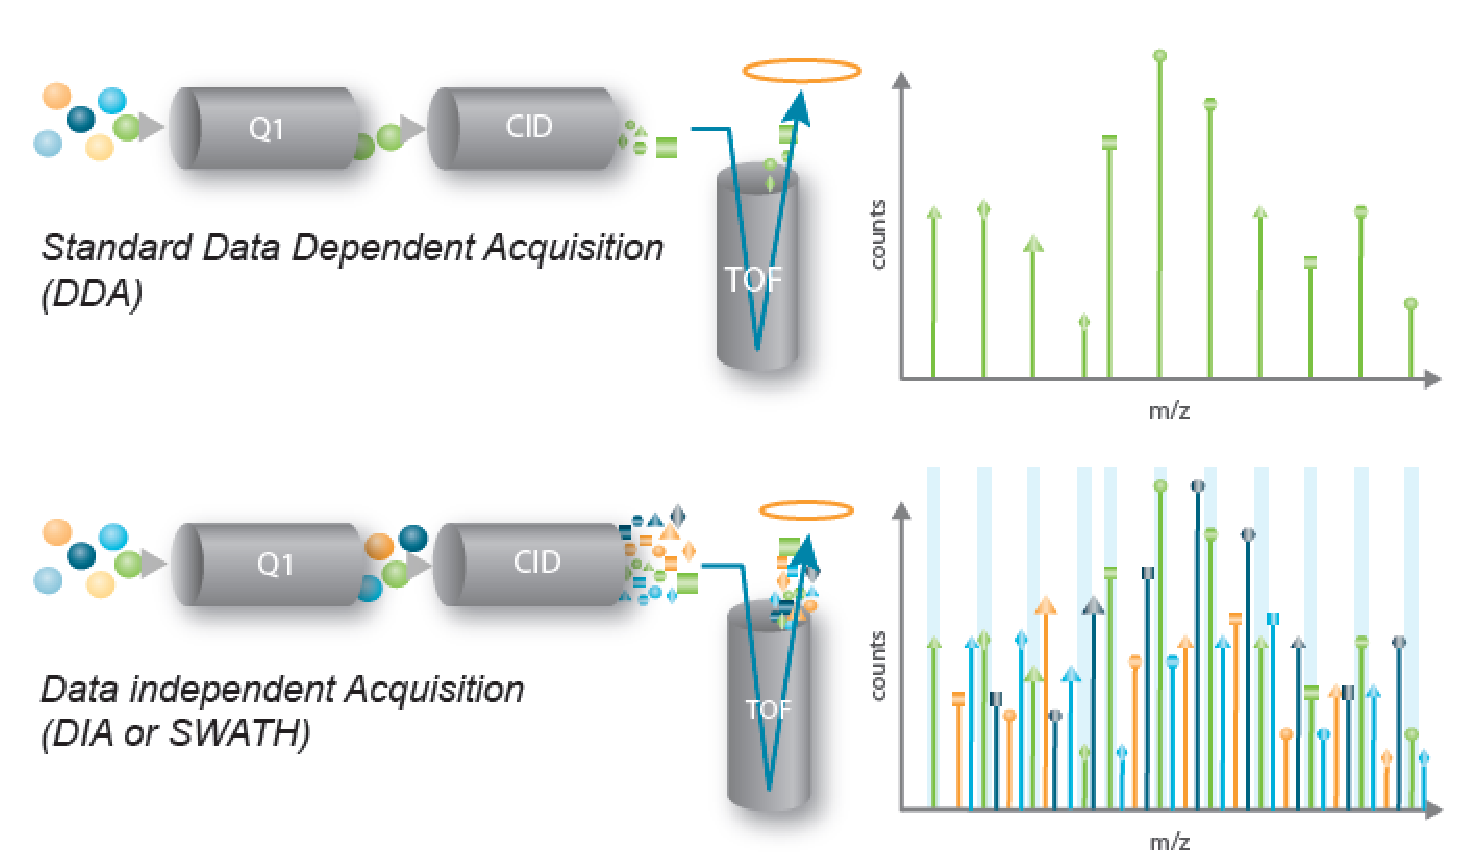
\includegraphics[width=.7\textwidth]{figures/figSwath.pdf}
%%    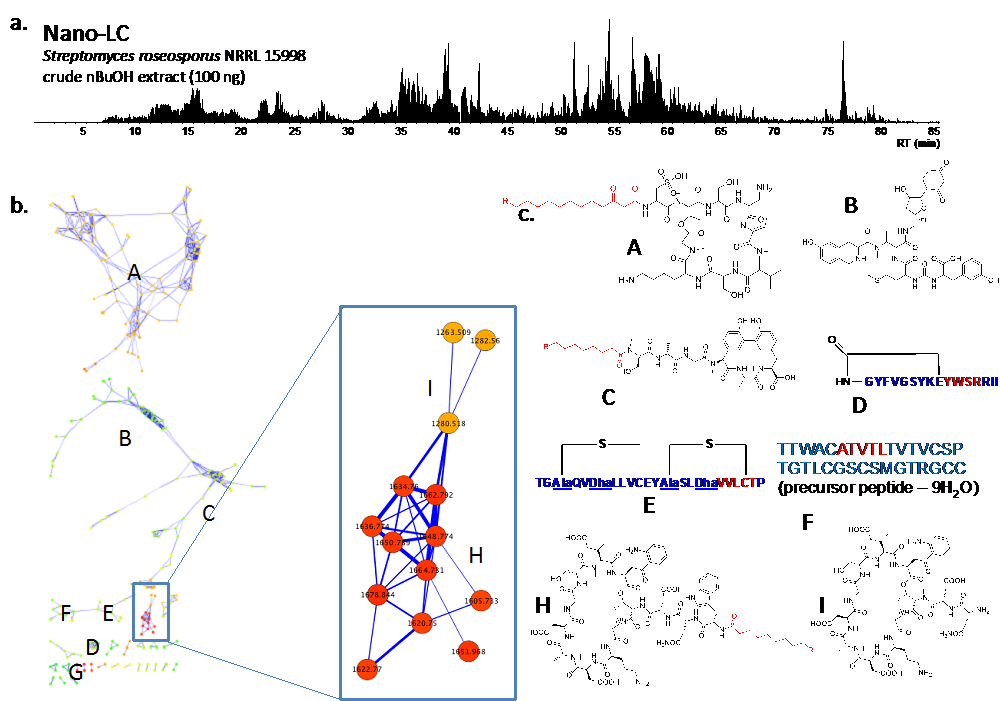
\includegraphics{figures/figApproach.png}
%  \caption{\footnotesize {\bf Differences between DDA and DIA mass spectrometry methods.} (top) In classical Data Dependent Acquisition (DDA), co-eluting peptides are first analyzed prior to fragmentation in a survey scan (MS1). The $n$ most abundant species are then sequentially isolated in the mass spectrometer, fragmented in the CID chamber and the fragment masses are measured in the TOF chamber. A typical MS/MS spectrum is shown on the right: these spectra are used for peptide identification. (bottom) In Data Independent Acquisition (DIA, here SWATH), there is no decision to select ions for fragmentation based on a precursor scan. Instead, the Q1 filters ions by relatively large mass windows: co-filtered peptides are co-fragmented in the CID chamber and co-analyzed in the TOF chamber. This results in a mixed spectrum, shown on the right, from which identification and quantification information can be retrieved using bioinformatics tools. The process is rapid such that the entire mass range can be analyzed in ~3 seconds.}
%  \label{fig.dbp.gingras.swath}
%\end{figure}

%*******************************************
\section{Approach}
%*******************************************

%\NeedRevision{(3) Approach: Describe methods and procedures to be used, emphasizing the relationship between the DBP and BTRC personnel and technologies, rationale for the proposed approach to the problem and impact of the expertise of the BTRC investigators and technology on the project.}

{\bf Determining specificity of bromodomains for acetyl-lysine residues.} The Gingras laboratory has already established a static interactome surrounding 77 of the acetylome components, each epitope tagged (FLAG) and expressed at near endogenous levels in human cells. Following affinity purification and mass spectrometry, ~3000 high-confidence interactions were detected that cover ~900 proteins. This constitutes the baseline interactome, which is then used to monitor the changes in interaction profiles associated with mutations (point mutations, translocations) and following cell perturbation, for example using the bromodomain-specific inhibitors (this will be done by SWATH). This interactome map is critical to understanding the processes in which bromodomain-containing proteins and other acetylome components are acting; however, how the recognition of the acetylated lysine by the bromodomain is related to the interactome is unclear at this point. To begin to characterize interactome specificity, this DBP will apply a multi-pronged approach to identify acetylation-dependent interactions, both in the context of recombinantly-expressed isolated bromodomains (tested both on synthetic peptides, on purified histones and on cell extracts), but also with full length proteins expressed in human cells. A key element of this strategy is to be able to identify acetylation sites directly from immunoprecipitates of bromodomain-containing proteins. %To start, we have modified our mChIP strategy to add, after the tryptic digest, an additional affinity step consisting of an anti-KAc pulldown at the peptide level.
% and analysis on a high mass resolution mass spectrometer.
We first tested
This approach was tested on the bromodomain-containing protein BRPF3, a component of the MOZ/MORF histone acetyltransferase complex. In addition to the known BRPF3 interaction partners, new interactors for this protein were also identified. The KAc enrichment approach also revealed acetylation sites on BRPF3 itself, and on many of its interactors.
%While several of these sites were present in a public repository (PhosphoSitePlus.org), 15 were new and thus highlight the %sensitivity of this approach.
%Mass spectrometric identification of acetylated sites was optimized by analyzing fractions of the same purification on different %mass spectrometers (and in the case of the Orbitrap Velos by employing different modes of fragmentation).
Importantly, this showed that - in comparison to a proteome-wide study of acetylation - the targeted study of the acetylome facilitates the identification of polyacetylated peptides. This is an important result, especially in light of recent results where the Gingras lab demonstrated that some of the bromodomains exhibit a preference for polyacetylated sites and that this preference may contribute to the recognition of histone code marks. %It is also noteworthy that many of the KATs (especially those of the MYST family) require auto-acetylation for activity. As such, being able to identify and study these critical residues is important. We have also developed approaches to determine the specificity of recombinant isolated bromodomains against synthetic peptides and histone preparations.

While the static interactome work described above was employing Data Dependent Acquisition (DDA) to discriminate between true and false positive interactions, this approach proved insufficiently sensitive to capture mutation- or treatment-induced changes in association.  
%Furthermore, the approach is not appropriate for quantification at the peptide level, which is what is required for the identification of the acetylated peptide specificity.
%
The Gingras laboratory has developed affinity purification (AP) methods in the past to successfully quantify interactome changes~\cite{choi10,breitkreutz10,filippakopoulos12}. But since a faster method was needed to rapidly probe multiple interactome components across varied conditions, they collaborated with AB SCIEX to develop a DIA-based AP-SWATH approach, which was first validated on known regulated interactions. This pipeline was then used to analyze changes in the BET family interaction profiles imparted by treatment with the JQ1 inhibitor. As expected based on the mode of action of the pharmacological compound, association of BRD3 with histones was markedly decreased, while interaction with several other proteins was maintained, indicating that they are not mediated by the KAc-bromodomain interaction. Surprisingly, new interaction partners were found to be enriched following JQ1 treatment, suggesting new links to DNA damage and transcription. Similar data were obtained for other BET family members, with JQ1 and other inhibitors. In these experiments, the analysis of SWATH data was accomplished by %a targeted data extraction strategy
using a spectral library built from the same samples by standard DDA.

In collaboration with CCMS, this DBP will extend this approach to i) aggregate all DDA runs into a spectral library that can be used for analysis of any SWATH run (interacts with TRD3), ii) develop methods for peptide identification (instead of just quantification) by spectral library and database searching of SWATH spectra (interacts with TRD3 and TRD7) and iii) develop methods for identification of modified peptides for which only the unmodified or less-modified version of the peptide is present in either a database or the spectral library (interacts with TRD3 and TRD7).

As a direct extension of this work, this DBP will also combine the use of chemical crosslinkers to explore the structural organization within protein complexes: proof of principle experiments in the Gingras laboratory have successfully crosslinked several complexes using BS3 and DSP (TRD7). The SWATH approach should be more sensitive than the previously employed DDA acquisition and thus enable a more extensive characterization of the intra- and intermolecular contacts in our protein complexes.

In collaboration with CCMS, we have already begun investigating fragmentation patterns for linked peptides using SWATH. Combining crosslinking with SWATH will enable identification of direct interaction partners, thereby facilitating the selection of proteins to follow-up in co-crystal studies. At the same time, knowledge of the interacting regions provided by AP-crosslinker-SWATH will permit the selection of the appropriate regions to analyze structurally, which is critical in this project in which many of the proteins are extremely large (upwards of 200kDa) and not possible to express recombinantly in amounts sufficient for crystallography. The data already planned for acquisition in this funded project will be ideal for these TRDs because it contains validated identifications of modified peptides (e.g., the subset of quantifiable peptides from Figure~\ref{fig.dbp.gingras.ptms}) but also provides opportunities for potentially discovering new modified peptides or new interaction partners as we become able to directly search SWATH spectra instead of limiting their use to peptide quantification only.

%\NeedRevision{CCMS PTMs - Need to be able to reproduce these discoveries directly from the data for all interactomics studies. This is perfect validated dataset for methods development.}
%
%{\bf Development of new methods for accurate mass spectrometry-based quantification} An important aspect of the proposal is our ability to accurately quantify interactions regulated by the recognition of the acetylation site (e.g. from a parallel purification of a wild-type bromodomain containing protein and a mutant in which the acetyl-lysine recognition is prevented). Furthermore, we wish to monitor the enrichment of acetylated peptides and quantify their relative abundance. While we and others have used several different quantitative proteomics approaches, including isotopic labeling approaches such as SILAC, and label-free approaches such as spectral counting and intensity measurement of the precursor ion in the mass spectrometer (so-called MS1 quantitation), here we propose to use quantification methods based on the intensity of the product ions in the MS/MS spectrum. We have previously used single reaction monitoring (SRM) to monitor changes in interactomes accurately and with high sensitivity (Appendix 5). Since SRM method building (i.e. the selection of the best precursor ions and daughter ions to monitor) is time-consuming, we have also developed (in collaboration industrial partner AB SCIEX, letter appended) a modified approach called MRMHR, which accelerates the development of quantification assays while providing the same accuracy
%on quantification. Lastly, we have implemented a data-independent quantification approach called SWATH which enables us to determine � again with high accuracy � the relative abundance of every identified species in a given dataset. Since the SWATH approach is very recent, we benchmarked it here to determine its efficiency in measuring interactome
%differences on cancer-associated mutations; this type of sample is very similar to what we are proposing to monitor in this proposal. AP-MS with SWATH quantification reveals differences between the interactions established by wild type CDK4 (cyclin dependent kinase 4) and two point mutants identified in melanoma that act in a dominant manner. As expected, we could readily detect the disruption of the interaction between the mutants and the cyclin dependent inhibitors of the INK family. Interestingly, however, we could also quantify increased interactions between the mutants and components of the HSP90 chaperone complex (suggesting folding issues with the mutants), and with another class of CDK inhibitor. These novel changes were validated by immunoblotting, confirming the usefulness of the approach. Importantly, quantification is accurate at the peptide level, which will enable us to monitor changes in acetylation. Further, the instrument on which we are performing SWATH measurements is the same as that used for acetylation site mapping, the AB-SCIEX TripleTOF 5600, ensuring the compatibility of our platform.
%
%\NeedRevision{CCMS Multiplexing}
%
%%**************************************************************************************
%% ------------------------------------------------------------------------------------
%\section{Technology Research and Development projects (TR\&Ds)}
%% ------------------------------------------------------------------------------------
%%**************************************************************************************
%
%This DBP will drive and substantially benefit from the proposed CCMS research and development on identification of spectra from modified peptides (TRD3), cross-linked peptides (TRD4) and multiplexed spectra (TRD7). In addition, the likely complexity of the resulting software and the expected volume of data to be processed will further drive the need for the proposed ProteoSAFe developments and MassIVE resources proposed here (TRD8).

\paragraph{Impact of the expertise of the CCMS investigators on DBP.} Drs. Bafna, Bandeira and Pevzner have extensive experience in the development of algorithms for analysis of PTMs~\cite{tsur05,bandeira07pnas,na11} and new types of MS data~\cite{kim09msdict,kim10cidetd}. In addition, Dr. Bandeira led the development of the first approach for multiplexed spectral library search~\cite{wang10} and the MixDB~\cite{wang11} database search for multiplexed spectra, which is computationally very similar to database search of cross-linked peptide spectra. Dr. Bandeira also led the development of the ProteoSAFe platform which already enabled the analysis of over 1 billion spectra and thus has the  expertise to implement the new search workflows in Gingras' laboratory.

% For all 3 aims

\bibliographystyle{plain}
\bibliography{../../bibtex/msms,../../bibtex/bandeiraLab,../../bibtex/immunology}
\end{document}
